\documentclass[xcolor=svgnames,smaller,draft]{beamer}
\usepackage[utf8]{inputenc}
\usepackage[T1]{fontenc}
\usepackage[english]{babel}
\usepackage{xspace}
\usepackage{amsmath}
\usepackage{amsthm}
\usepackage{mathtools}
\usepackage{bm}
\usepackage{booktabs}
\usepackage{microtype}
\usepackage[version=3]{mhchem}
\usepackage{siunitx}

\usepackage{tikz}
\usetikzlibrary{decorations.pathmorphing}
\tikzset{font=\small} % Samme fontstørrelse i TikZ som i figurtekst
\usepackage{pgfplots}
\pgfplotsset{compat=1.6}

\usepackage[sc]{mathpazo}
\renewcommand{\ttdefault}{txtt}
\usepackage{url}
\urlstyle{rm}

%% Custom commands:

% Afledte, partielle og ej, der alle tager to argumenter (som
% \frac). \diff er almindeligt afledt én gang og \ddiff er to gange -
% begge med oprejste(!) hårde d'er. \pdiff er partielt afledt én gang
% og \ppdiff to gange.
\newcommand\pdiff[3][\partial]{\frac{#1 #2}{#1 #3}}
\newcommand\ppdiff[3][\partial]{\frac{#1^2 #2}{#1 #3^2}}
\newcommand\ddiff[2]{\pdiff[\mathrm{d}]{#1}{#2}}
\newcommand\dddiff[2]{\ppdiff[\mathrm{d}]{#1}{#2}}

% Kommando til at lave parenteser på begge sider
\newcommand\paren[1]{\left(#1\right)}

% Random convenience.
\newcommand{\inv}{^{-1}}             % "I minus første"
\newcommand{\idx}[1]{_{\textup{#1}}} % Tekst-indeks med få tastetryk.
\newcommand{\order}[1]{^{\textup{(#1)}}} % Orden
\newcommand{\half}{\frac{1}{2}}


\mode<presentation>{
  \usetheme[compress]{Singapore}
  \usecolortheme[named=MidnightBlue]{structure}
  \useinnertheme{circles}
  \usecolortheme{orchid}
  \setbeamertemplate{blocks}[rounded]
  \usefonttheme{serif}
  \usefonttheme{professionalfonts}
  \usefonttheme[onlylarge]{structurebold}
  \setbeamerfont{block title}{series*=m}
  \setbeamercolor{example text}{fg=Maroon}
}

\title{Nonlinear optics}
\subtitle{Wave mixing and the Kerr effect}
\author{
  Anders Aspegren Søndergaard \\
  Kristoffer Theis Skalmstang \\
  Michael Munch \\
  Steffen Videbæk Fredsgaard \\
}
\date{March 12, 2014}

%------------------------------------------------------------------------
% Set depth of table of content
%------------------------------------------------------------------------
\setcounter{tocdepth}{1}

\AtBeginSection[] {
  \begin{frame}<beamer>
    \frametitle{Outline}
    \tableofcontents[currentsection]
  \end{frame}
}

\begin{document}

% \begin{frame}
%   \frametitle{Typografitest}
%   Tekst
%   \begin{itemize}
%   \item Punkt
%   \end{itemize}
%   \begin{block}{block}
%     Hest
%   \end{block}
%   \begin{example}
%     example
%   \end{example}
% \end{frame}
% \end{document}

\frame{\titlepage}
\section{Nonlinear optics}





\begin{align*}
  \label{eq:wave-general}
  \nabla^2 \mathbf E - \frac{1}{c^2} \ppdiff{\mathbf E}{t}
  = \frac{1}{\epsilon_0c^2} \ppdiff{\mathbf P}{t},
\end{align*}

\[
\mathbf P = \epsilon_0 ( \chi\order1 \mathbf E +
\chi\order2 \mathbf E^2 + \chi\order3 \mathbf E^3 \dots )
\]







%%% Local Variables: 
%%% mode: latex
%%% TeX-master: "nonlinearslides"
%%% End: 

\chapter{Three-wave mixing}
\label{cha:mixing}


The Three-wave mixing is a property of the second order non-linearity of the polarity dependence of the electric field, $\mathcal{E}(t)$. 
It is a phenomenon where the two waves mix together to a third. 



\section{Mathematical formulation}
\label{sec:mixing-math}

To qualitatively examine the interaction between the two electromagnetic waves, of frequencies $\omega_1$ and $\omega_2$ with electric field amplitude $\mathcal{E}_1  \equiv \mathcal{E}(\omega_1)$ and $\mathcal{E}_1  \equiv \mathcal{E}(\omega_1)$ respectively, a superposition of these monochromatic plane waves is composed: 
\[
\mathbf{\mathcal{E}}(t) = \Re (\mathcal{E}_1e^{i(\mathbf{k_1} \cdot \mathbf{r} - \omega_1 t)}+\mathcal{E}_2e^{i(\mathbf{k_2} \cdot \mathbf{r} \omega_2 t)}),
\]
and put into the second order part of the polarity expansion \cite{saleh}
\begin{align*}
     \mathbf{P}^{NL} & = \varepsilon_0 \chi^{(2)} \mathbf{E}^2(t) \\
&= \varepsilon_0 \chi^{(2)} 2 \Re \left[
\left(|E_1|^2+|E_2|^2\right)e^{0} + |E_1|^2e^{i2(\mathbf{k_1} z - \omega_1t)}+|E_2|^2e^{i2(\mathbf{k_2} z - \omega_2t)} \right.\\
& \left. +2E_1E_2e^{i((\mathbf{k_1} + \mathbf{k_2}) \cdot \mathbf{r} - (\omega_1+\omega_2)t)}  +2E_1E_2^*e^{i((\mathbf{k_1} - \mathbf{k_2}) \cdot \mathbf{r} - (\omega_1-\omega_2)t)} \right].
\end{align*}
Since this gives feedback to the electromagnetic field new frequencies are generated; $0$, the uninteresting one, $2\omega_1$ and $2\omega_2$, which are the original frequencies second harmonics, and more interesting, the sum and difference of the initial frequencies. The last two frequency couplings are often referred to as up- and down-conversion respectively.

It is clear that for the up- and down-conversion the third wave frequency will be:
\[
\omega_3 = \omega_1 \pm \omega_2
\]
and that a further phase matching constraint on the wave vector is necessary,
\[
\mathbf{k}_3 = \mathbf{k}_1 \pm \mathbf{k}_2,
\]
for a strong feedback in electric field change. Which phy





\section{Numeric formulation}
\label{sec:mixing-numeric}

\begin{align}
P = 
\end{align}


Example KDP crystal

Notes:
four wave frequency wave mixing of higher order

%%% Local Variables: 
%%% mode: latex
%%% TeX-master: "nonlinear"
%%% End: 

\begin{frame}
  \frametitle{Kerr effect: Mathematical formulation}

  With a centrosymmetric and isotropic medium the important term is
  \[
  \mathbf P = \epsilon_0 ( \chi\order1 \mathbf E +
  {\chi\order2 \mathbf E^2} + \textcolor{red}{\chi\order3 \mathbf E^3} \dots )
  \]
\end{frame}

\begin{frame}
  \frametitle{Suspectibility}

  The refractive index of the medium will then be intensity dependent. 
  \begin{align*}
    n &= \sqrt{1 + \chi_1 + \chi_3 |\mathcal{E}|^2}\\
    &\simeq n_0 + \tfrac{1}{2} n_2 |\mathcal{E}|^2,
  \end{align*}
\end{frame}

\begin{frame}
  \frametitle{Gaussion beams}
  Assume: Beam has a gaussian shape

  $\Rightarrow$ Refractive index is peaked at center.
  {\centering
  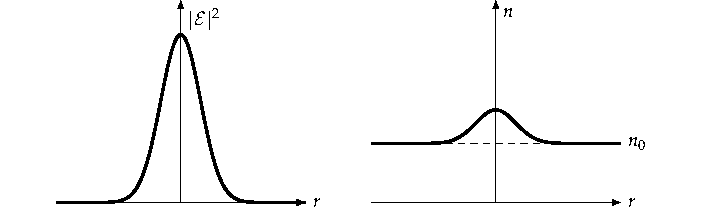
\includegraphics[width=1\columnwidth]{gaussrefrac}}

This is effectively a positive lens that will focus the beam. 
\end{frame}

\begin{frame}
  \frametitle{Waveequation}
  Assume: Monocromatic linear polarized plane wave.
  \[E = \mathcal{E}(x,y) e^{-i (\omega t-kz)}\]
  Insert into to the wave equation
\[  \nabla^2 E - \frac{1}{c^2} \ppdiff{E}{t}
  = \frac{1}{\epsilon_0c^2} \ppdiff{P}{t}\]
  This gives the nonlinear wave equation:

  \[\nabla^2 \mathcal{E} + \frac{\omega^{2}}{c^2} \mathcal{E} = - \frac{\omega^2}{\epsilon_0 c^2} \left( \epsilon_0 \chi_1
    \mathcal{E} + \epsilon_0 \chi_3 |\mathcal{E}|^2 \mathcal{E}
  \right).\]

  which is a partial differential equation !
\end{frame}


%%% Local Variables: 
%%% mode: latex
%%% TeX-master: "nonlinearslides"
%%% End: 

\begin{frame}
  \frametitle{Solving partial differential equations}
  
\end{frame}


%%% Local Variables: 
%%% mode: latex
%%% TeX-master: "nonlinearslides"
%%% End: 

\begin{frame}
  \frametitle{First year optics: A simple optical fibre}

  Step index optical fibre utilizing total internal reflection
  \begin{itemize}
  \item core of material with refractive index $n_1$
  \item outer shell of material with refractive index $n_2 < n_1$
  \end{itemize}
  Acceptance angle is $\sin\theta\idx{max} = \sqrt{n_1^2 - n_2^2}$
  when assuming $n=1$ outside the fibre.

  \begin{center}
    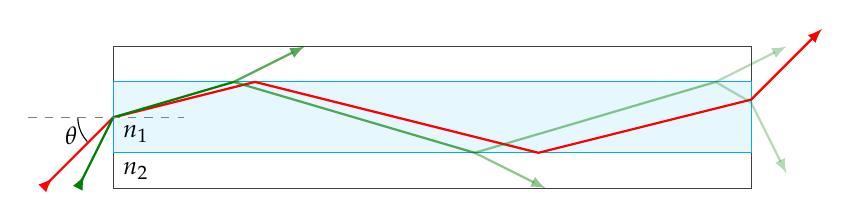
\begin{tikzpicture}[scale=0.9]
      \draw[thin,black!75] (2,-1) rectangle +(9,2);
      \fill[cyan!10,draw=cyan,thin] (2,-.5) rectangle +(9,1);
      \draw[thick,red,latex reversed-latex]
        (1,-1) -- (2,0) -- ++(2,.5) -- ++(4,-1) -- ++(3,.75) -- ++(1,1);
        \begin{scope}[green!50!black,thick]
        \draw[thick,latex reversed-]
          (1.5,-1) -- (2,0) -- (3.7,.5);
        \draw[thick,opacity=.66] (3.7,.5) -- (7.1,-.5);
        \draw[thick,opacity=.66,-latex] (3.7,.5) -- +(1,.5);
        \draw[thick,opacity=.44] (7.1,-.5) -- (10.5,.5); 
        \draw[thick,opacity=.44,-latex] (7.1,-.5) -- +(1,-.5);
        \draw[thick,opacity=.29,-latex] (10.5,.5) -- (11,.21) -- +(.5,-1);
        \draw[thick,opacity=.29,-latex] (10.5,.5) -- +(1,.5);
      \end{scope}
  
      \node[anchor=south west] at (2,-.5) {$n_1$};
      \node[anchor=north west] at (2,-.5) {$n_2$};
      
      \draw[thin,dashed,gray] (.8,0) -- (3,0);
      % node[above,at start,anchor=south west] {Normal};
      \draw[thin] (1.5,0) arc (180:223:.5)
      node[left,anchor=east,yshift=2pt] {$\theta$};
    \end{tikzpicture}
  \end{center}

  Trivially, rays with angle of incidence greater than the acceptance
  angle of the fibre will be lost.
\end{frame}


\begin{frame}
  \frametitle{Better fibres: Graded-index}

  Graded-index fibre (wide industrial usage)
  \begin{itemize}
  \item refractive index varies radially, maximal at the center
  \item does not rely on total internal reflection
  \end{itemize}
  Rays are gradually refracted towards the axis, where the refraction
  index is maximal. Here too, the fibre has a certain acceptance.

  \begin{center}
    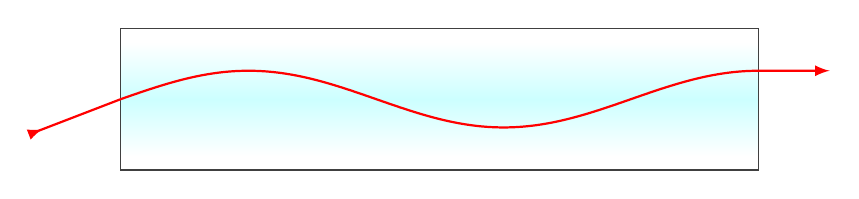
\begin{tikzpicture}[scale=0.9]
      \shade[top color=white,bottom color=white,middle color=cyan!20]
        (2,-.8) rectangle +(9,1.6);
      \draw[thin,black!75] (2,-1) rectangle +(9,2);
      \draw[thick,red,latex reversed-latex] (.7,-.5) -- (2,0) sin (3.8,.4)
       cos (5.6,0) sin (7.4,-.4) cos (9.2,0) sin (11,.4) -- +(1,0);
      % \fill[cyan!10,draw=cyan,thin] (2,-.5) rectangle +(9,1);
      % \draw[thick,red,latex reversed-latex]
      %   (1,-1) -- (2,0) -- ++(2,.5) -- ++(4,-1) -- ++(3,.75) -- ++(1,1);
      %   \begin{scope}[green!50!black,thick]
      %   \draw[thick,latex reversed-]
      %     (1.5,-1) -- (2,0) -- (3.7,.5);
      %   \draw[thick,opacity=.66] (3.7,.5) -- (7.1,-.5);
      %   \draw[thick,opacity=.66,-latex] (3.7,.5) -- +(1,.5);
      %   \draw[thick,opacity=.44] (7.1,-.5) -- (10.5,.5); 
      %   \draw[thick,opacity=.44,-latex] (7.1,-.5) -- +(1,-.5);
      %   \draw[thick,opacity=.29,-latex] (10.5,.5) -- (11,.21) -- +(.5,-1);
      %   \draw[thick,opacity=.29,-latex] (10.5,.5) -- +(1,.5);
      % \end{scope}
  
      % \node[anchor=south west] at (2,-.5) {$n_1$};
      % \node[anchor=north west] at (2,-.5) {$n_2$};
      
      % \draw[thin,dashed,gray] (.8,0) -- (3,0);
      % % node[above,at start,anchor=south west] {Normal};
      % \draw[thin] (1.5,0) arc (180:223:.5)
      % node[left,anchor=east,yshift=2pt] {$\theta$};
    \end{tikzpicture}
  \end{center}
  For a parabolic index profile rays follow sinusoidal paths, with
  paths and acceptances generally determined by the index profile and
  beam intensity profile.

\end{frame}


\begin{frame}
  \frametitle{Qualitative description of the Kerr effect}

  \begin{itemize}
  \item In an optical fibre, the refractive index i fixed upon
    manufacture. Conversely, the refractive index in a Kerr-medium is
    \alert{induced} by the electrical field of the propagating laser.

  \item The qualitative description of the propagating light is
    similar, as individual rays sees an effective refractive index
    depending on the rays particilar value of the electric field.

  \item For gaussian beams, the electric field depends on the distance
    from the beam axis and beam waist. Hence, the effective refractive
    index varies for certain parts of the beam.
  \end{itemize}
\end{frame}


\begin{frame}
  \frametitle{Self-focusing}

  \begin{itemize}
  \item Self-focusing takes place when the induced refractive index is
    sufficiently high, ie. for beams and parts thereof with high
    intensity.

  \item At low intensity the induced refractive index is insufficient
    to overcome diffractive spreading. At very high intensity the
    materiale breaks down.

  \item For a gaussian beam inverse focal length (dioptic power) is
    determined by the beam parameters and the nonlinear component of
    the refractive index of the Kerr-medium
    \begin{align*}
        f\idx{kerr}\inv = \frac{4}{\pi} \frac{n_2 P}{w_0^4} z,
    \end{align*}
    where $z$ is the distance traveled in the medium.

  \item Major advantage: Optical axis is induced by the beam.
  \end{itemize}

\end{frame}


%%% Local Variables: 
%%% mode: latex
%%% TeX-master: "nonlinearslides"
%%% End: 


\end{document}

%%% Local Variables: 
%%% mode: latex
%%% TeX-master: t
%%% End: 
